\documentclass{article}

% set font encoding for PDFLaTeX or XeLaTeX
\usepackage{ifxetex}
\ifxetex
  \usepackage{fontspec}
\else
  \usepackage[T1]{fontenc}
  \usepackage[utf8]{inputenc}
  \usepackage{lmodern}
  \usepackage{graphicx}
\fi

% used in maketitle
\title{
        \begin{center}
        
\includegraphics[width=8cm]{Unison.png}
        \end{center}
        \newline
       Reporte Actividad 2}
\author{José Alberto "Buma" Burruel Martinez}
\date{7 de Febrero del 2018}

% Enable SageTeX to run SageMath code right inside this LaTeX file.
% documentation: http://mirrors.ctan.org/macros/latex/contrib/sagetex/sagetexpackage.pdf
% \usepackage{sagetex}

\begin{document}
\maketitle{
            \begin{center}
            Introducción a Phyton, Jupyter y Pandas
            \end{center}
            }

\newpage

\section{Introducción}
En esta actividad nos dimos una breve introducción a lo que es Python y le herramienta de graficación Pandas y Matplotlib, todo esto en el area de trabajo de Jupyter.

\section{Desarrollo}
\subsection{Algo chilo}
Primeramente, las características padres del lenguaje de programación Python es que se basa en poder importar paquetes de trabajo para utilizarlos como herramientas en el código que queremos utilizar, de la misma manera en la que se hacen los documentos en \LaTeX . Por ejemplo, Pandas y Matplotlib son paquetes que nos ayudan a procesar los datos que queremos manejar y graficar dichos datos analisados en el Data Frame, respectivamente.


Otra de las características interesantes es que el código se va creando por secciones que sirven para unicamente una sola actividad, llamadas celdas, las cuales se van compilando conforme avanzas en el código con otra celda. Digamos que quieres ver la relacion entre dos variables de las que tienes en la base de datos. Lo primero que debes hacer es cargar el archivo en una celda y compilar, siguiente celda debes declarar el manejo de datos, y por fin en otra celda hacer el código para graficar las variables y listo, la gráfica se despliega directamente en el area de trabajo

\subsection{Algo malo}
El unico inconveniente que podría verle a este sistema de trabajo es que, ya que maneja directamente las gráficas, tablas, etc, es que el tamaño del archivo puede convertirse un poco muy grandes.

\subsection{¿Qué hicimos?}
Inicialmente, trabajamos con una base de datos que contienen mediciones de sondeos atmosféricos, cuyos resultados presentaremos a continuación.

\subsubsection{Analisis de datos}
Primero hicimos un análisis que describiera los datos de las variables del archivo.

    \begin{center}
    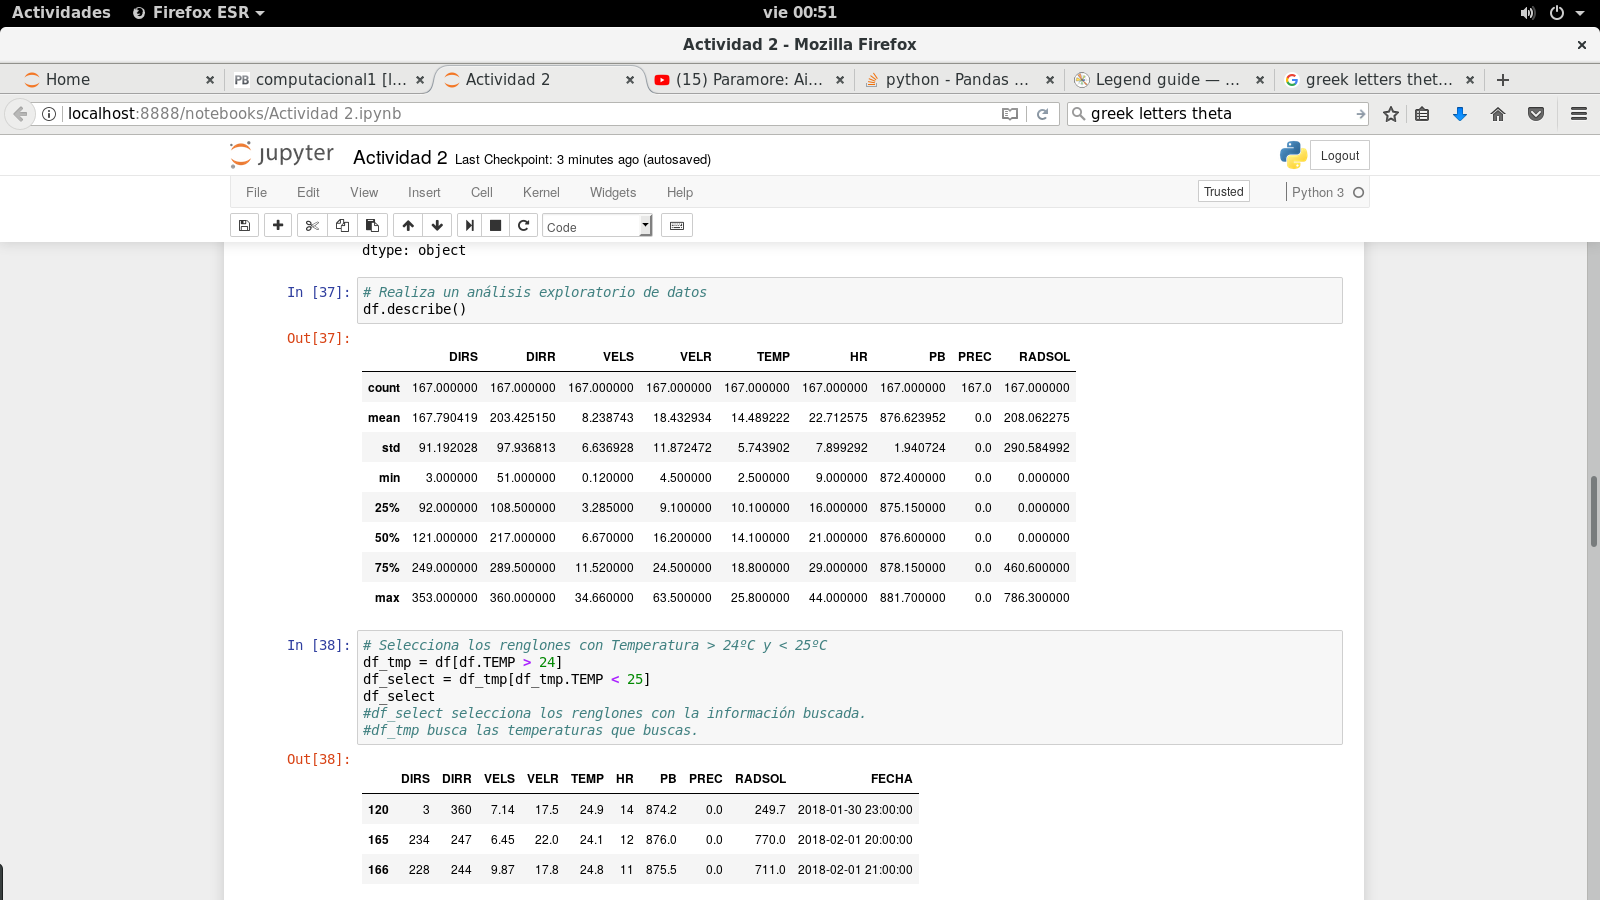
\includegraphics[width=20cm]{Analisis.png}
    \end{center}

\subsubsection{Graficas}
Lo siguiente en la lista era hacer una lista de gráficas, las cuales mostraré de inmediato:

    \begin{figure}

    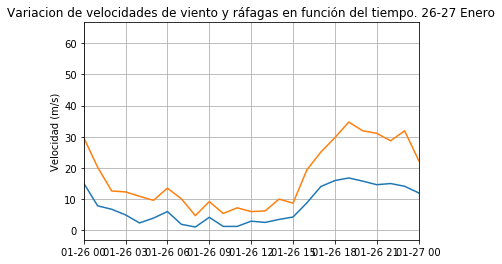
\includegraphics[width=10cm]{Velocidades contra Fecha.png}
    \caption{Grafica de velocidad contra la fecha.}


    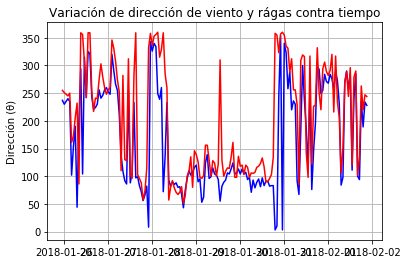
\includegraphics[width=\linewidth]{Direcciones contra Fecha.png}
    \caption{Grafica de la dirección del viento y de las ráfagas contra fecha}

    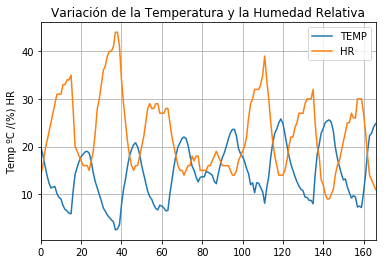
\includegraphics[width=10cm]{HR contra Temp.png}
    \caption{Gráfica de Humedad Relativa contra Fecha}
    
    \end{figure}
    
 \newpage
    
    \begin{figure}
    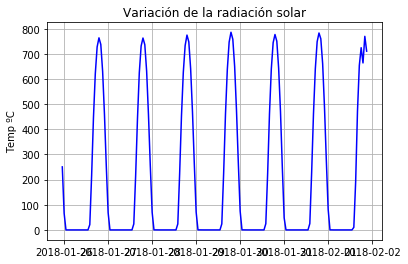
\includegraphics[width=10cm]{RadSol contra Fecha.png}
    \caption{Radiación Solar contra la fecha}

    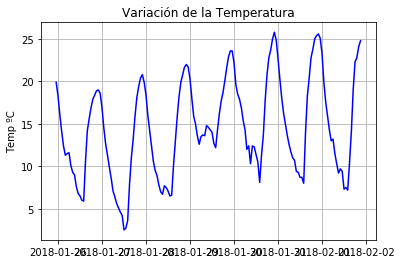
\includegraphics[width=10cm]{Temp contra fecha.png}
    \caption{Temperatura contra fecha}

    \end{figure}
    
\newpage

\section{Apéndice}
\subsection{¿Cuál es tu primera impresión de Jupyter Notebook?}
Que se ve bastante sencillo de utilizar, pero sí tiene su ciencia detrás de todo.
\subsection{¿Se te dificultó leer código en Python?}
Casi no, está bastante sencillo una vez que le agarras el rollo y encuentras los patrones.
\subsection{¿En base a tu experiencia de programación en Fortran, que te parece el entorno de trabajar en Python?}
Pues obviamente es diferente ya que Python es más como lenguaje de traducción en vivo, pero se ve muy padre.
\subsection{A diferencia de Fortran, ahora se producen las gráficas utilizando la biblioteca Matplotlib. ¿Cómo fue tu experiencia?}
Mucho más facil, gracias al cielo <3 
\subsection{En general, ¿qué te pereció el entorno de trabajo en Python?}
Está curado, loco UuU
\subsection{¿Qué opinas de la actividad? ¿Estuvo compleja? ¿Mucho material nuevo? ¿Que le faltó o que le sobró? ¿Qué modificarías para mejorar? }
Pues, sirve de buena introducción. Bastante sencilla, la verdad.
\subsection{¿Comentarios adicionales que desees compartir?}
Que debería hacer los reportes la misma semana y no un domingo en la noche :S
    
\end{document}
